\begin{figure}[ht]
	\centering
	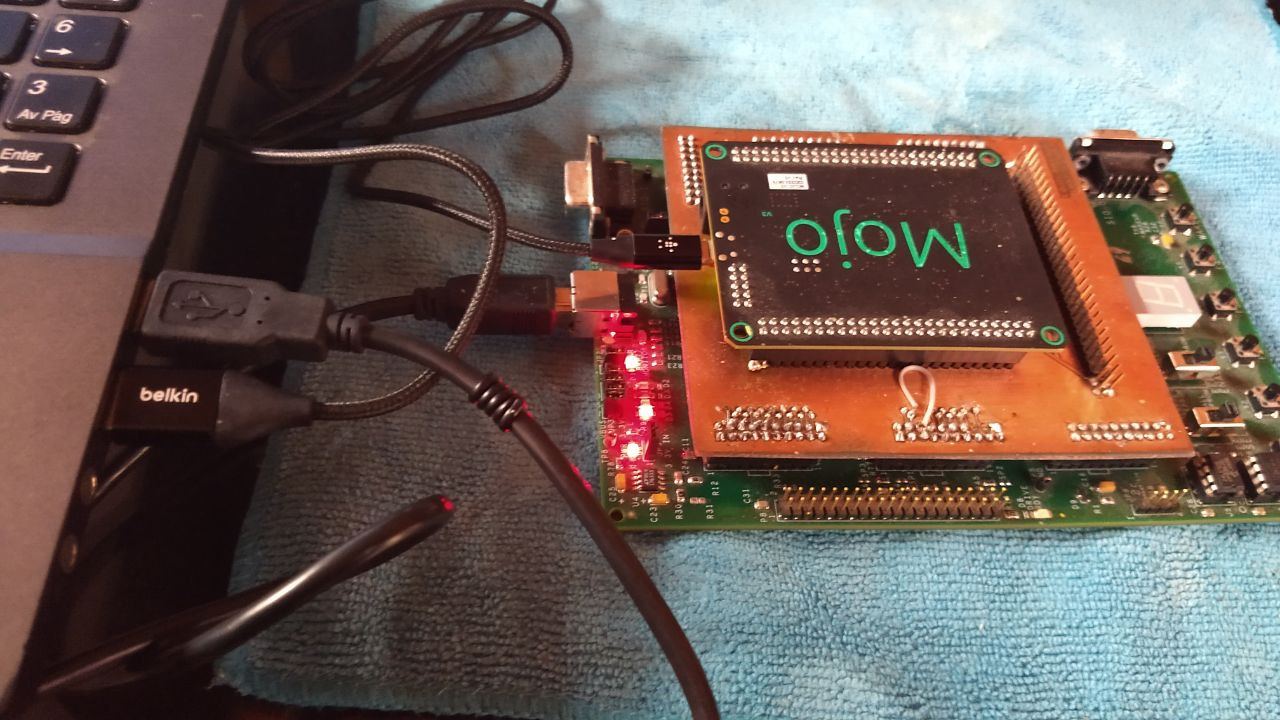
\includegraphics[width=0.7\textwidth]{sistema2.jpg}
	\caption{El sistema desarrollado en funcionamiento}
	\label{test:todo}
\end{figure}

Como se muestra en la Figura \ref{test:todo}, en el sistema completo, montado y en funcionamiento, el \acrshort{fpga} es conectado a la interfaz \acrshort{usb} través de la Placa de Interconexión. A su vez, la interfaz \acrshort{usb} se enlaza con la \acrshort{pc} a través de un cable. La conexión entre la interfaz \acrshort{usb} con la \acrshort{pc} sirve no solo para transferir los datos que llegarán el \acrshort{fpga}, sino también el programa que ejecutará el controlador FX2LP.

Además, el \acrshort{fpga} también se conecta a la \acrshort{pc} a través de un cable con el propósito de transferirle el archivo de programación y de proveerle alimentación a través del puerto \acrshort{usb}.
Con los dispositivos dispuestos en la configuración descripta, se procedió a cargar los diferentes programas elaborados para cada uno de ellos y finalmente, se ejecutó el programa de pruebas.
El programa de pruebas fue ejecutado por más de 24 horas con el objetivo de tener una buena cantidad de datos estadísticos como para probar la robustez del sistema, como así también su tasa de transferencia.
Todas las transferencias, tanto de entrada como de salida a la \acrshort{pc} fueron guardas en un archivo de registro, documentando la fecha, el sentido de la comunicación y los datos intercambiados. 